\documentclass[12pt]{article}
%\documentclass{article}
\usepackage{amsmath,amsthm,amssymb}
\usepackage{enumerate}

\usepackage[english]{babel}
 \usepackage{graphicx}
 \usepackage[usenames,dvipsnames,svgnames,table]{xcolor}
\usepackage{palatino}

\usepackage{fancyhdr}
\pagestyle{fancy}
\fancyhf{}
\rhead{Instructor: David Dobor}
\lhead{CIS 2033, Spring 2017, Homework 2}
\rfoot{Page \thepage}


\newenvironment{question}[2][Question]{\begin{trivlist}
\item[\hskip \labelsep {\bfseries #1}\hskip \labelsep {\bfseries #2.}]}{\end{trivlist}}
\newenvironment{answer}[2][Answer]{\begin{trivlist}
\item[\hskip \labelsep {\bfseries #1}\hskip \labelsep {\bfseries #2.}]}{\end{trivlist}}

\begin{document}

\subsection*{\centering{Homework 2}}
\centering\textcolor{teal}{\\ (  Due at 11 AM on Thursday, February 2 )}
\vspace{5mm}


 \begin{question}{1} We roll two fair 6-sided dice. Each one of the 36 possible outcomes is
assumed to be equally likely.
\begin{enumerate}[(a)]
 \item  Find the probability that doubles were rolled.
\item  Given that the roll resulted in a sum of 4 or less, find the conditional probability
that doubles were rolled.
 \item Find the probability that at least one die is a 6.
 \item Given that the two dice land on different numbers, find the conditional probability
that at least one die is a 6.
 \end{enumerate}

\end{question} 

%\vspace{5mm}

\pagebreak
 \begin{question}{2} Let the sample space be the 4 $\times$ 4 square, $\Omega  = [0, 4]^2$, in the real plane. Let the probability 
 of a set in $\Omega$ be 1/16-th of the area of that set (that is, assume the uniform probability law on $\Omega$). Let $A$ be 
 the set of points $(x, y) \in [0, 4]^2$ for which $y \leq x$. Let $B$ be the set of points for which $x \leq 3$. Find $P(A \mid B)$.
\end{question} 


 

\pagebreak
 \begin{question}{3} At a certain stage of a criminal investigation, the inspector in charge is 60
  percent convinced
of the guilt of a certain suspect. Suppose, however, that a \emph{new} piece of evidence
which shows that the criminal has a certain characteristic (such as left-handedness,
baldness, or brown hair) is uncovered. If 20 percent of the population possesses this
characteristic, how certain of the guilt of the suspect should the inspector now be if it
turns out that the suspect has the characteristic?
\end{question} 



%\vspace{5mm}
\pagebreak
 \begin{question}{4} A ball is drawn at random from an urn containing one red and one white ball. If the white ball is drawn, it is put back into the urn. If the red ball is drawn, it is returned to the urn together with two more red balls. Then a second draw is made. What is the probability a red ball was drawn on both the first and the second draws.
\end{question} 


\pagebreak
 \begin{question}{5} \ 
 \begin{enumerate}[(a)]
 \item  Suppose that a shuttle's launch depends on three key devices that operate independently of each other and malfunction with probabilities 0.01, 0.02, and 0.02, respectively. If any of the key devices malfunctions, the launch will be postponed. Compute the probability for the shuttle to be launched on time, according to its schedule.
 \item There's a 1\% probability for a hard drive to crash. Therefore, it has two backups, each having a 2\% probability to crash, and all three components are independent of each other. The stored information is lost only in an unfortunate situation when all three devices crash. What is the probability that the information is saved?
 \end{enumerate}
 

\end{question} 

%\vspace{5mm}
\pagebreak
 \begin{question}{6}   Start your \texttt{python} interpreter and answer the following questions. Unlike your answers to the other problems 
 in this assignment, the answers to this question need not be explained - simply write down or circle your final answer.  
\begin{enumerate}[(a)]
 \item Use \texttt{random.choice} and \texttt{range} to generate a random integer from 0-9. Enter your code in your \texttt{python} interpreter. What's the result?\item What will \texttt{random.choice(list([1,2,3,4]))} produce?
     \begin{enumerate}[(A)]
         \item \texttt{list([1,2,3,4])}
         \item \texttt{[1,2,3,4]}
         \item A value from 1-4 , selected at random
         \item This code contains an error.
      \end{enumerate}
 \item Which of the following lines of code sums random integers from 0-9?
      \begin{enumerate}[(A)]
         \item \texttt{sum(random.sample(range(10),10))}
         \item \texttt{sum(random.choice(range(10),10))}
         \item \texttt{random.sample\_sum(range(10),10)}
         \item \texttt{sum(random.choice(range(10)) for i in range(10))}
      \end{enumerate}
 \end{enumerate}
\end{question} 




\end{document}





\begin{align}
&P(A) + P(A^c) + P(B) = P(A \cup A^c \cup B) \\
&P(A) + P(B) \leq 1 \\
&P(A^c) + P(B) \leq 1 \\
&P(A \cup B \cup C) \geq P(A \cup B)
\end{align}


\begin{enumerate}[(a)]
 \item What is $P(Z = 3)$?
\item What is $P(U = 3)$?
 \item What is $P(S \text{ is even })$?
 \end{enumerate}



%%%%%%%%%%%%%%%%%%%%%%%%%%%%% OLD QUESTIONS %%%%%%%%%%%%%%%%%%%%%%%%%%%%%

 \begin{question}{2} A coin is tossed twice. Alice claims that the event of two heads is at least as likely if we know that 
 the first toss is a head than if we know that at least one of the tosses is a head. 
 \begin{enumerate}[(a)]
 \item  Is she right? (try to answer this without peeking into parts (b), (c), and (d) of this question.)
 \item Assume the coin is fair, i.e. all outcomes $\{HH, HT, TH, TT \}$ are equally likely. Let $A$ be the event that the first toss is a head, and $B$ be the event that the second toss is a head. What are - in words - the events $A \cap B$  and "$A \cap B$ given $A$"? Compute $P(A \cap B \mid A)$. 
 \item With the same assumptions and notation as in the previous part, what is the event  "$A \cap B$ given $A \cup B$"? Compute $P(A \cap B \mid A \cup B)$.
 \item Compare the results you got in parts (b) and (c).
 \item  Was Alice right? 
 \item Does it make a difference if the coin is fair or unfair?
 \end{enumerate}
\end{question} 



 \begin{question}{4} A ball is drawn at random from an urn containing one red and one white ball. If the white ball is drawn, it is put back into the urn. If the red ball is drawn, it is returned to the urn together with two more red balls. Then a second draw is made. What is the probability a red ball was drawn on both the first and the second draws.
\end{question} 


%\vspace{5mm}
\pagebreak
 \begin{question}{5} Tom Walker is a tightrope walker who's taking CIS 2033. 
 At a recent campus party he decides to showcase his talents to some of his classmates. Tom carefully lays down his unfinished bottle of beer, quickly rigs up his equipment, and begins his stunning performance. 

\vspace{2mm}
\ \ \ \ Tom manages to keep his balance, but takes a step forward with probability $p$ and takes a step back with probability $(1 - p)$.
 
  \begin{enumerate}[(a)]
 \item What is the probability that after two steps, Tom will be at the same place on the rope as where he started?
 \item What is the probability that after three steps, Tom will be one step forward from where he started?
 \item Given that after three steps he has managed to move ahead one step, what is the probability that the first step he took was a step forward?
 \end{enumerate}
 \textit{Hint (a possible way to model Tom's behavior):} One of Tom's classmates suggests to model Tom's performance by using a tree similar to what she's seen in class (shown below). Here $F$ stands for the event "Tom takes a step $F$orward", and $B$ stands for the event "Tom takes a step $B$ackward". 
 
 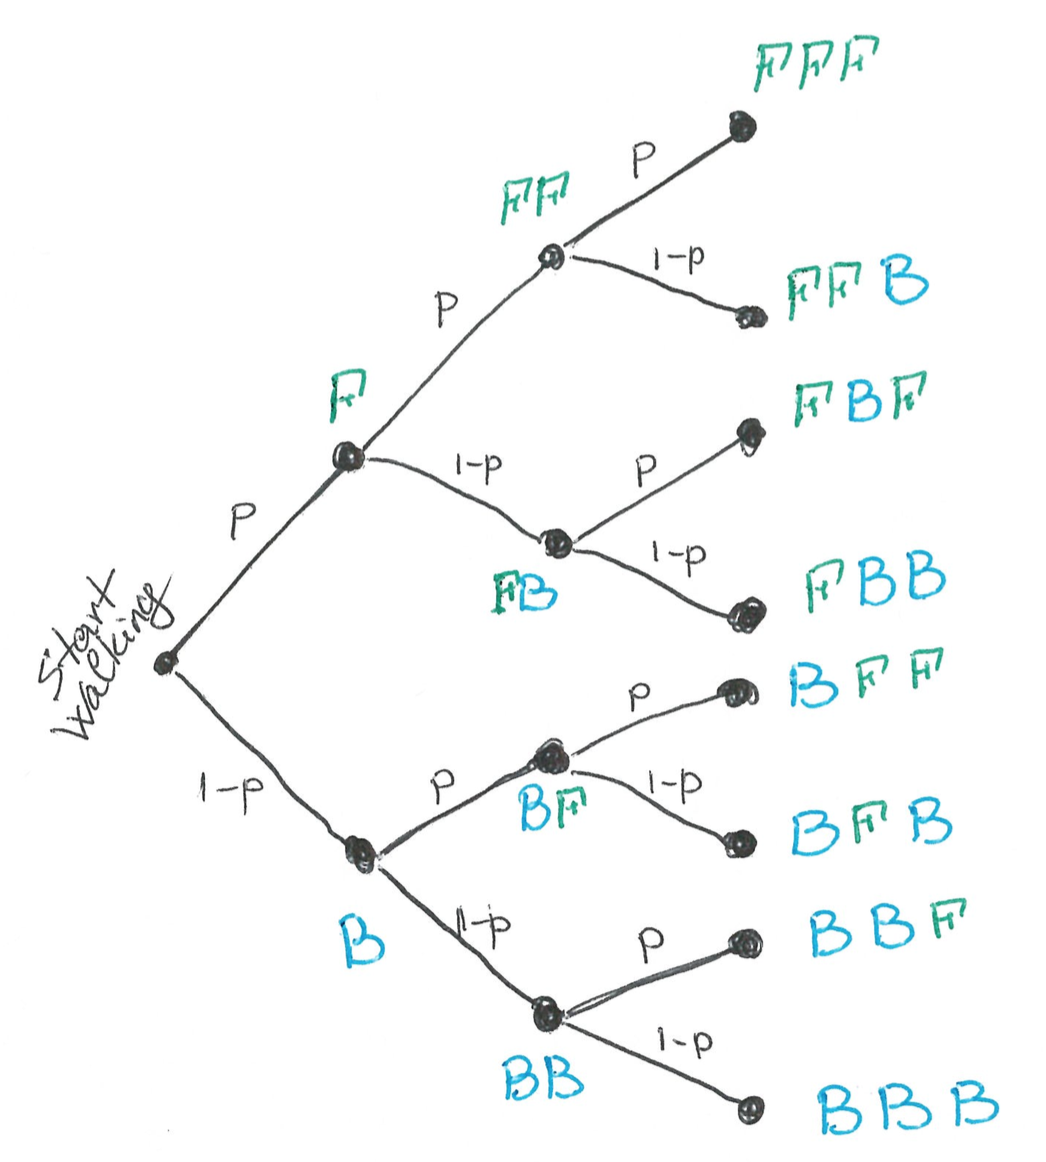
\includegraphics[scale=0.4]{Walker}
 
 
 
 
\end{question} 



